\documentclass[prez_tpt]{subfiles}
\begin{document}

% Intro section
\begin{frame}[t]
%\vskip-1em
\frametitle{$Z$-step: Sparse coding}
$\rightarrow \pmb D$ fixed, update $Z$
\[
Z^{[n],*} = \argmin_{Z^{[n]}}\| X^{[n]} - \sum_{k=1}^K\pmb D_k *  Z_k^{[n]}\|_2^2
+ \lambda\| Z^{[n]}\|_1
\]
\strongpoint{Independent for each $n\in\llbracket1, N\rrbracket$}
\vskip1em
%
\underline{\textbf{Related Algorithms:}}\\[.5em]
\begin{itemize}%\itemsep.5em
    \item Iterative Soft-Thresholding Algorithm (ISTA)\\\mycite{Daubechies2004, Chalasani2013}
    \item Fast ISTA \\\mycite{Beck2009, Wohlberg2016}
    \item Alternated Direction Method of Multiplier (ADMM)\\\mycite{Gabay1976, Bristow2013}
    \item Coordinate Descent (CD) \\\mycite{Friedman2007, Kavukcuoglu2013}
\end{itemize}
\end{frame}

%---------------------------------------------------------------------------
\subsection{LGCD}
%---------------------------------------------------------------------------

\begin{frame}[t]{Coordinate Descent (CD)}
	
	Minimize
    %
	\[
    	Z^{*} = \argmin_{Z}\| X - \sum_{k=1}^K\pmb D_k *  Z_k\|_2^2
    			+ \lambda\| Z\|_1
	\]
    %
	Update one coordinate at each iteration.\\[1em]
	\begin{enumerate}
		\item Select a coordinate $(k_0, t_0)$ to update.
		\visible<2->{ \item Compute a new value $Z'_{k_0}[t_0]$ for this coordinate}
	\end{enumerate}

\only<1>{
	Three algorithms for LASSO:
	\begin{itemize}\itemindent1em
		\item Cyclic updates; $\bO{1}$  \mycite{Friedman2007}
		\item Random updates; $\bO{1}$ \mycite{Nesterov2010}
		\item Greedy updates; $\bO{KL}$ \mycite{Osher2009}
	\end{itemize}
}
\only<2>{
	For convolutional CD, we can use optimal updates:
	$$
		Z'_{k_0}[t_0] = \frac{1}{\|\pmb D_{k_0}\|_2^2}\textbf{ST}(\beta_{k_0}[t_0], \lambda),
	$$
	with {\small $\textbf{ST}(y, \lambda) = \text{sign}(y)(|y| - \lambda)_+$}.
	\cite{Kavukcuoglu2013} showed this can be done efficiently, with $\mathcal O(KL)$ operations.
}
\only<3>{
    \strongpoint{Converges to the optimal point for CSC problem in $\bO{\frac{1}{q}}$ iterations.}
    
    \vskip1em
    Trade-off between cheap computational complexity (random/cyclic CD) and importance sampling with faster convergence (Greedy CD).\\\mycite{Nutini,Karimireddy2018}
}
\end{frame}




\begin{frame}{Locally Greedy Coordinate Descent \citeconfright{Moreau2018}{ICML}}


We introduced the LGCD method which is an extension of GCD.\\
{
    \centering
    \inputTikZ{.7}{LGCD}
}

\only<1-2>{
    \vskip1em
    GCD has $\mathcal O(K\widetilde{T})$ computational complexity.\\[1em]
    \only<2>{But the update itself has complexity $\mathcal O(KL)$}
}
%
\visible<3->{
    With a partition $\mathcal C_m$ of the signal domain $[1, K]\times [0, \widetilde{T}[$,
    \[
    \mathcal C_m = [1, K]\times [\frac{(m-1)\widetilde{T}}{M}, \frac{m\widetilde{T}}{M}[
    \]%
}%
\visible<4->{%
    The coordinate to update is chosen greedily on a sub-domain $\mathcal C_m$\\[1em]
    
    {\centering$\frac{\widetilde{T}}{M} = 2L-1~~\Rightarrow~~\mathcal O$(Coordinate selection) = $\mathcal O$(Coordinate Update)\\[1em]}
    
    The overall iteration complexity is $\mathcal O(KL)$ instead of $\mathcal O(K\widetilde{T})$.
    \strongpoint{Efficient for sparse $Z$}
}


\end{frame}

\begin{frame}{Fast optimization}
Comparison of the coordinate selection strategy for CD on simulated signals\\
We set $K=10$, $L=150$, $\lambda = 0.1 \lambda_{\max}$\\[1em]
\centering
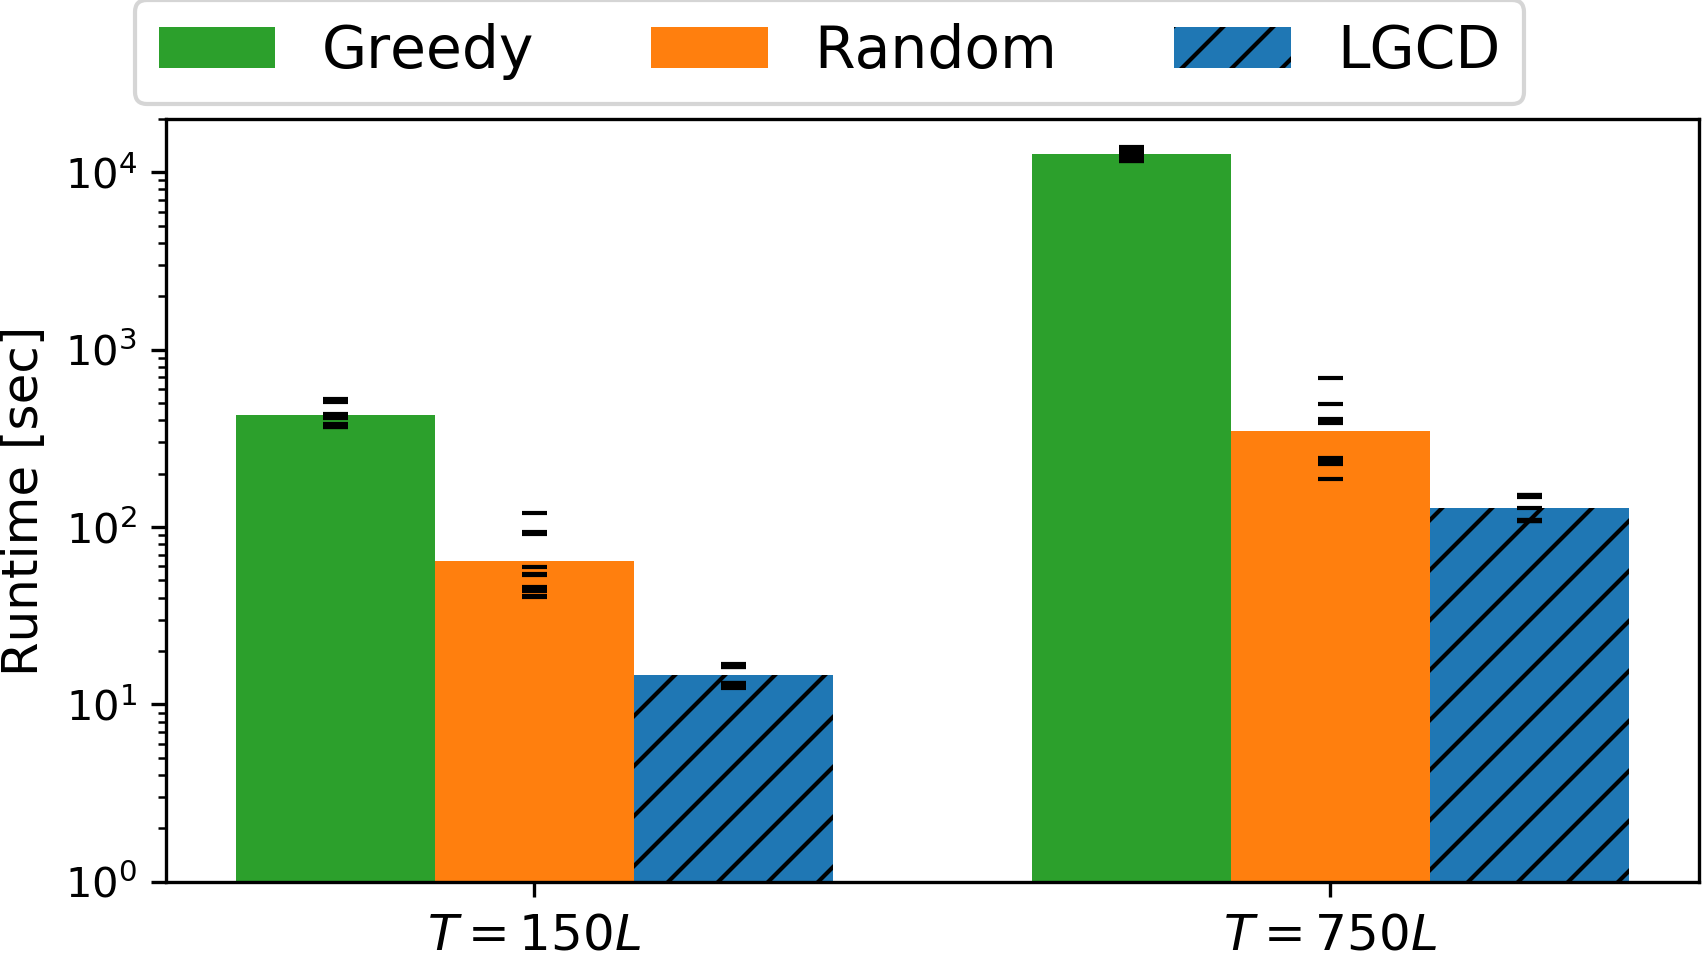
\includegraphics[width=.9\textwidth]{CD_strategies_comparison.png}
\end{frame}




%---------------------------------------------------------------------------
\subsection{DICOD}
%---------------------------------------------------------------------------


\begin{frame}{Weak dependence of the coordinate updates}
The update of the $W$ coordinates $(k_w, \omega_w)_{w=1}^W$ with additive update $\Delta Z_{k_w}[\omega_w]$ changes the cost by:
\begin{align*}
\Delta E =
\overbrace{\sum_{i=1}^W\Delta E_w}^{
    \text{iterative steps}}
- \underbrace{\sum_{w \neq w'}(d_{k_w} * d_{k_{w'}}^\Lsh)[\omega_{w'} - \omega_w]
    \Delta Z_{k_w}[\omega_w] \Delta Z_{k_{w'}}[\omega_{w'}]}_{
    % \Delta Z_{k_w}[w] \Delta Z_{k_{w'}}[w']}_{
    \text{interference}}, \label{eq:interf}
\end{align*}

\strongpoint{If the updates are far enough, they can be considered as independent.}
\end{frame}

\begin{frame}{Distributed Convolutional Coordinate Descent\\\citeconfright{Moreau2018}{ICML}}

{
\centering
\inputTikZ{.7}{DICOD}\\
}
\vskip1em
\begin{itemize}[<+->]\itemsep1em
\item Split the coordinates in continuous sub-segment
$\mathcal S_w = \left[\frac{(w-1)T}{W}, \frac{wT}{W}\right[$.
\item Use CD updates in parallel in each sub-segment.
\item Notify neighbor workers when the update is on the border of $\mathcal S_w$.
\item What do we do when two updates are interfering?
\end{itemize}

\end{frame}



\begin{frame}{DICOD convergence \citeconfright{Moreau2018}{ICML}}
\setbeamercolor{my title}{bg=primary!60, fg=secondary}
\setbeamercolor{my body}{bg=white, fg=black}

DICOD converges to the solution of the CSC for 1D signals without having a control mechanism on the interference.\\[1em]

\begin{beamerboxesrounded}[upper=my title,lower=my body,shadow=true]{
        \usebeamerfont{block title}Theorem (Convergence of DICOD)}
    We consider the following assumptions:\\[.3em]
    {\bf H1: }
    If the cross correlation between atoms of $\pmb D$ is strictly smaller than 1.\\[.3em]
    {\bf H2: }
    No cores stop before all its coefficients are optimal.\\[.3em]
    {\bf H3: }
    If the delay in communication between the processes is inferior to the update time.\\[1em]
    Under these assumptions, the DICOD algorithm converges asymptotically to the
    optimal solution $Z^*$ of CSC.
\end{beamerboxesrounded}

\end{frame}

\begin{frame}{Distributed Convolutional Dictionary Learning (DiCoDiLe-Z)\\\citeconfright{Moreau2019}{preprint}}

\begin{columns}[c]
    \column{.5\textwidth}
    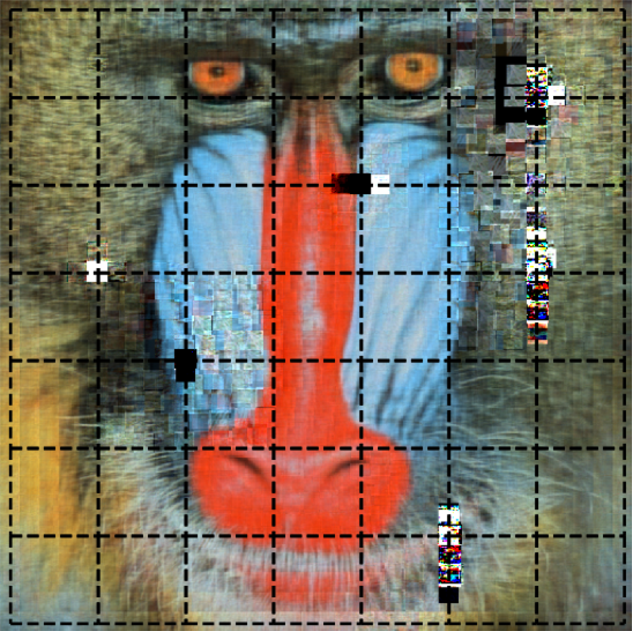
\includegraphics[width=.9\textwidth]{soft_lock_M49_support16}
    \column{.5\textwidth}
    \begin{itemize}[<+->]\itemsep1em
        \item DICOD does not work for higher dimensional signals.
        \item Extension require to control interferences. 
        \item Use asynchronous mechanism: Soft-lock.
    \end{itemize}
\end{columns}

\end{frame}



%\begin{frame}{Distributed Convolutional Dictionary Learning (DiCoDiLe-Z)}
%\vskip1em
%\begin{columns}[c]
%\column{.35\textwidth}
%\begin{itemize}\itemsep1em
%\only<1>{
%\item Update candidate $\omega_0$ is independent of other workers as
%\[
%\mathcal V(\omega_0) \subset \mathcal S_w
%\]
%}
%
%\only<2>{
%\item Update candidate $\omega_1$ impacts $\mathcal S_{w+1}$
%\[
%\mathcal V(\omega_1) \not\subset \mathcal S_w
%\]
%\item It is accepted only is no better update is possible in the "soft-locked" area.
%\item Need to notify $\mathcal S_{w+1}$.
%}
%\only<3>{
%\item Updates in $\omega_2$ need to notify worker $w$ to maintain consistent estimate in the border zone $\mathcal B_L(\mathcal S_w)$.
%
%\item Low communication: decentralized and below 1ko.
%}
%\end{itemize}
%\column{.65\textwidth}
%\inputTikZ{.75}{Sw_dicod.tex}
%\end{columns}
%\end{frame}


%---------------------------------------------------------------------------
\subsection{Complexity Analysis}
%---------------------------------------------------------------------------


\begin{frame}{Numerical speed-up}

\centering
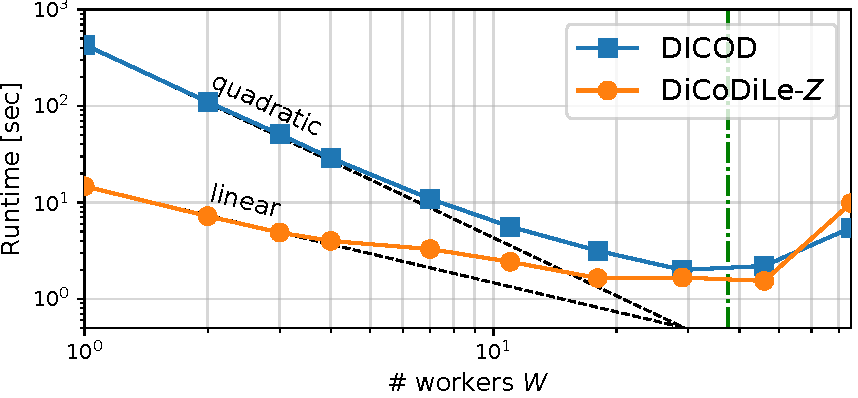
\includegraphics[width=\textwidth]{scaling_T150}
\\
\large Running time as a function of the number of workers $W$.

\end{frame}



%%%%%%%%%%%%%%%%%%%%%%%%%%%%%%%%%%%%%%%%%%%%%%%%
%   Conclusion
%%%%%%%%%%%%%%%%%%%%%%%%%%%%%%%%%%%%%%%%%%%%%%%%

\begin{frame}{Recap Part II}

	\textbf{Take home message}\\[.5em]
	\begin{itemize}\itemsep.5em
        \item LGCD is a very efficient algorithm when working with CSC for long signals.
		\item Can be distributed efficiently for multi-dimensional signals,
		\item Good scaling properties with the number of workers $W$ used to distribute the algorithm.
	\end{itemize}
	\vskip1.5em
	
	\textbf{Ahead of us}\\[.5em]
	\begin{itemize}\itemsep.5em
		\item Extend this algorithm to local penalization such as Group LASSO.
        \item This algorithm could be used for algorithm such as MP for $\ell_0$ or $\ell_{0,\infty}$ penalties.
	\end{itemize}
\end{frame}

\biblio{}
\end{document}